%lwarp%\begin{lateximage}[two points inside a rectangle joined by a continuous path][][width: 50\%;]
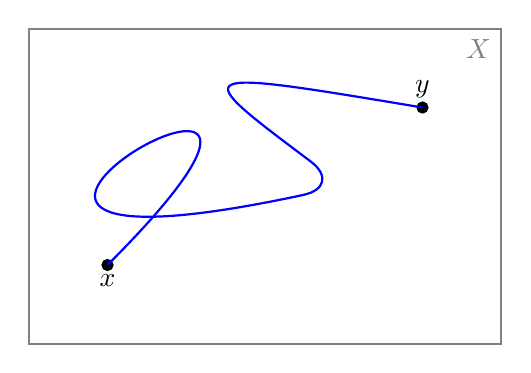
\begin{tikzpicture}
	
	% Draw the topological space X as a rectangle
	\draw[thick, gray, use as bounding box] (0, 0) rectangle (6, 4) node[anchor=north east] {$X$};
	
	% Define points x and y
	\filldraw (1, 1) circle (2pt) node[anchor=north] {$x$};
	\filldraw (5, 3) circle (2pt) node[anchor=south] {$y$};
	
	% Draw a continuous curve connecting x and y
	\draw[thick, blue, rounded corners=15pt] 
	(1, 1) .. controls (5, 5) and (-3, 0.5) .. (4, 2) .. controls (2, 3.5) .. (5, 3);
	
\end{tikzpicture}

\begin{tikzpicture}
	\draw (0,0) circle(3pt) node[anchor=north, yshift=-2pt] {$p$};
	\draw[shorten >= 3pt] (-5,0) -- (0,0);
	\draw[shorten >= 3pt] (5,0) -- (0,0);
\end{tikzpicture}


		%lwarp%\begin{lateximage}[a horizontal line and a vertical line inside a square X times Y][][width: 40\%;]
		\begin{tikzpicture}
			\def\ybase{0.4}
			\def\myx{1.2}
			\def\myy{3.7}
			\def\myxprime{3.9}
			\def\myyprime{1.6}
			
			
			\draw[line width=6pt, green, opacity=0.5] (\myxprime,\ybase) -- (\myxprime,5);
			\node[green!50!black, anchor=south] at (\myxprime,5) {$\{x_2\}\times Y$};
			\draw[line width=6pt, cyan, opacity=0.5] (0,\myy) -- ++(6,0);
			\node[cyan!50!black, anchor=west] at (6, \myy) {$X \times \{y_1\}$};

			
			\draw (0,\ybase) -- (6,\ybase) node[midway, anchor=south]{$X$};
			\draw (0,\ybase) -- (0,5) node[midway, anchor=west]{$Y$};
			\draw (0,5) -- (6,5) -- (6,\ybase);
			
			\filldraw (\myx,\myy) circle(3pt) node[anchor=south]{$(x_1,y_1)$};
			\filldraw (\myxprime,\myy) circle(3pt) node[anchor=south west]{$(x_2,y_1)$};
			\filldraw (\myxprime,\myyprime) circle(3pt) node[anchor=west]{$(x_2,y_2)$};
			
			\draw[-{LaTeX}, shorten >= 3pt, thick] (\myx,\myy) -- 
			node[midway, anchor=north]{path} (\myxprime, \myy) ;
			\draw[-{LaTeX}, shorten >= 3pt, thick] (\myxprime,\myy) -- 
			node[midway, anchor=west]{path} (\myxprime, \myyprime) ;
			
		\end{tikzpicture}
		%lwarp%\end{lateximage}

